\documentclass[compress]{beamer}

\mode<presentation>
{
  %\usetheme{Warsaw}
  %\usecolortheme{spruce}
  % or ...
	%\useoutertheme{infolines}
  %\setbeamercovered{transparent}
  
  \usetheme{CambridgeUS}
    \setbeamercolor{item projected}{bg=darkred}
    \setbeamertemplate{enumerate items}[default]
    \setbeamertemplate{navigation symbols}{}
    \setbeamercovered{transparent}
    \setbeamercolor{block title}{fg=darkred}
    \setbeamercolor{local structure}{fg=darkred}
  
  % or whatever (possibly just delete it)
}

\usepackage{verbatim} 
\usepackage{listings}
\usepackage{tikz}
\usetikzlibrary{arrows}
\usetikzlibrary{shapes}
\tikzstyle{block}=[draw opacity=0.7,line width=1.4cm]

\newcommand{\bigpause}{\bigskip \pause}

\lstloadlanguages{C++}
\lstnewenvironment{code}
	{%\lstset{	numbers=none, frame=lines, basicstyle=\small\ttfamily, }%
	 \csname lst@SetFirstLabel\endcsname}
	{\csname lst@SaveFirstLabel\endcsname}
\lstset{% general command to set parameter(s)
	language=C++, basicstyle=\footnotesize\sffamily, keywordstyle=\slshape,
	emph=[1]{tipo,usa}, emphstyle={[1]\sffamily\bfseries},
	basewidth={0.47em,0.40em},
	columns=fixed, fontadjust, resetmargins, xrightmargin=5pt, xleftmargin=15pt,
	flexiblecolumns=false, tabsize=2, breaklines,	breakatwhitespace=false, extendedchars=true,
	numbers=left, numberstyle=\tiny, stepnumber=1, numbersep=9pt,
	frame=l, framesep=3pt,
}

\usepackage[spanish]{babel}
% or whatever

\usepackage[utf8]{inputenc}
% or whatever

\usepackage{times}
\usepackage[T1]{fontenc}
% Or whatever. Note that the encoding and the font should match. If T1
% does not look nice, try deleting the line with the fontenc.


\title[Geometr\'ia Computacional] % (optional, use only with long paper titles)
{Geometr\'ia Computacional}

\author[Melanie Sclar] % (optional, use only with lots of authors)
{~Melanie Sclar}
% - Give the names in the same order as the appear in the paper.
% - Use the \inst{?} command only if the authors have different
%   affiliation.
\institute[UBA] % (optional, but mostly needed)
{
  %\inst{1}%
  Facultad de Ciencias Exactas y Naturales\\
  Universidad de Buenos Aires
}
\date[PAP] % (optional, should be abbreviation of conference name)
{Problemas, Algoritmos y Programación}

% Ac¿ se puede insertar el logo de la UBA
% \pgfdeclareimage[height=0.5cm]{university-logo}{university-logo-filename}
% \logo{\pgfuseimage{university-logo}}



% Delete this, if you do not want the table of contents to pop up at
% the beginning of each subsection:
\AtBeginSubsection[]
{
  \begin{frame}<beamer>{Contenidos}
    \tableofcontents[currentsection,currentsubsection]
  \end{frame}
}

\newcommand{\be}{\begin{equation*}}
\newcommand{\ee}{\end{equation*}}
\newcommand{\state}[1]{\left|\,#1\,\right\rangle}
\newcommand{\costate}[1]{\left\langle\,#1\,\right|}
\newcommand{\trace}{\text{Tr}}
\newcommand{\su}{\uparrow}
\newcommand{\sd}{\downarrow}
\newcommand{\im}{\text{Im}}
\newcommand{\re}{\text{Re}}

% If you wish to uncover everything in a step-wise fashion, uncomment
% the following command:

%\beamerdefaultoverlayspecification{<+->}


\begin{document}
\pgfdeclarelayer{background}
\pgfsetlayers{background,main}
\begin{frame}
  \titlepage
\end{frame}

\begin{frame}{Contenidos}
  \tableofcontents
  % You might wish to add the option [pausesections]
\end{frame}

\section{Introducci\'on}
\begin{frame}

Generalmente, los problemas de geometr\'ia de ACM requieren calcular 
alguna cantidad (por ej., una distancia, un \'area, etc) relacionada con
elementos geom\'etricos como puntos, l\'ineas, c\'irculos, etc.
Para resolverlos, debemos poder ser capaces de:\\
\bigskip
\begin{enumerate}
\item Representar los objetos geom\'etricos involucrados en el problema, 
para poder operar con ellos.

\item Desarrollar un algoritmo para buscar la respuesta deseada.
\end{enumerate}

Entonces, para poder llegar a la segunda parte (la m\'as interesante), primero tenemos que ser capaces de llevar a cabo la primera.

\bigskip

\textbf{Aclaraci\'on:} Nos referiremos siempre a problemas en $\mathbb{R}^2$, ya que son los m\'as comunes.

\end{frame}

\section{Los elementos m\'as b\'asicos: puntos, vectores y rectas}
\begin{frame}[fragile]
Un punto en el plano (o un vector desde el origen hasta dicho punto) se puede representar con un par ordenado de coordenadas en un sistema cartesiano:

\begin{center}
$\vec{P} = (x,y)$ con $x,y \in \mathbb{R}$
\end{center}

\bigskip

Se puede representar como {\tt pair<double,double>}, pero es poco declarativo. Mejor hacer un {\tt struct}:

\begin{lstlisting}
struct Punto {
      double x;
      double y;
      // double z; para problemas en el espacio, etc.
};
\end{lstlisting}

\end{frame}

\subsection{Algunas operaciones importantes entre vectores}

\begin{frame}
\begin{itemize}
\item La suma y resta de vectores se realiza componente a componente:
    %
    \be
    \vec{P} = \vec{P}_1 \pm \vec{P}_2  \qquad \Longleftrightarrow \qquad (x, y) = (x_1 \pm x_2, y_1 \pm y_2)
    \ee
    \vspace{0.25cm}
    \item La longitud o \emph{norma} de un vector es $|\vec{P}| = \sqrt{x^2 + y^2}$.
\vspace{0.25cm}
    \item La distancia eucl\'idea entre dos puntos $\vec{P}_1$ y $\vec{P}_2$ es $|\vec{P}_1 - \vec{P}_2|$
\end{itemize}
\end{frame}

\begin{frame}{Producto escalar entre vectores}

\begin{block}{Producto escalar}
El \emph{producto escalar} de dos vectores $u = (x_1,y_1)$ y $v = (x_2,y_2)$ es un n\'umero, y se define como
    %
    \be
    \vec{u} \cdot \vec{v} = x_1 x_2 + y_1 y_2 = |\vec{u}| |\vec{v}| \cos\theta
    \ee
    \be
    \vec{u} \cdot \vec{v} = x_1 x_2 + y_1 y_2 + z_1 z_2 = |\vec{u}| |\vec{v}| \cos\theta \mbox{  (en 3D)}
    \ee
    %
\end{block}

\begin{itemize}
    \item El valor del producto escalar es la proyección ortogonal de $u$ sobre $v$, expresada con signo y multiplicada por $|v|$. Notar que como es conmutativo, lo mismo vale al revés.
    \item Observar que en particular si $\theta = 90^\circ$ el producto escalar se anula.
    \textbf{Es decir, dos vectores son perpendiculares si y s\'olo si su producto escalar da 0}.
\end{itemize}

\end{frame}

\begin{frame}{Producto cruz entre vectores}

El producto vectorial (o producto cruz) de dos vectores es un \emph{vector} en la direcci\'on normal al plano generado por ellos (¡esto puede ser muy \'util para problemas en $\mathbb{R}^3$!). \\

Si $u,v \in \mathbb{R}^2$ ($u = (x_1,y_1)$ y $v = (x_2,y_2)$), se define $u \times v$ como:
\be
   \vec{u} \times \vec{v} = (0, 0, x_1 y_2 - x_2 y_1)
\ee
Luego, es fácil deducir que:
\be
   |\vec{u} \times \vec{v}| = x_1 y_2 - x_2 y_1
\ee

y se puede demostrar que:

\be
    |\vec{u} \times \vec{v}| = |\vec{u}| |\vec{v}| \sin\theta,
\ee

y que adem\'as \textbf{ $|u \times v|$ es el \'area del paralelogramo determinado por los dos vectores.}
\end{frame}


\begin{frame}{Producto cruz entre vectores}

El signo del producto indica la orientaci\'on de los vectores.
%
\begin{center}
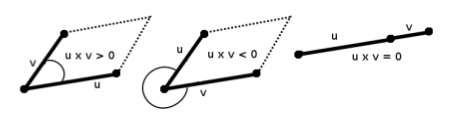
\includegraphics[scale=0.6]{images/producto_cruz.png}
\end{center}
%

Adem\'as, notemos que aqu\'i $u \times v = 0$ significa que los dos vectores tienen igual direcci\'on (¡no confundir con el producto escalar!). \\

\end{frame}

\subsection{Representaci\'on de recta y segmento}
\begin{frame}{¿C\'omo represento una recta?}

Una recta puede ser representada de m\'as de una forma: las dos m\'as usuales son:

\begin{itemize}
\item $L(x) = m x + b$, siendo $m$ la pendiente de la recta y $b$ la ordenada al origen.
\item $L(t) = \mathbf{p} + t \mathbf{v}$, siendo $\mathbf{v} \in \mathbb{R}^2$ el vector direcci\'on y 
$\mathbf{p}$ un punto en la recta. $t \in \mathbb{R}$ es un escalar que representa cu\'anto se dilata o contrae el vector $\mathbf{v}$.
\end{itemize}

El primer enfoque tiene una posible desventaja, ¿cu\'al es?

\bigpause
\invisible<1>{
La pendiente de una recta es un cociente entre dos n\'umeros, y por ende debemos asegurarnos que no se indefina dicho cociente. 
As\'i, si se quiere representar la recta vertical $x = c$, se la deber\'a tratar como un caso especial en el c\'odigo (¡Oh no, un $if$!).
}
\end{frame}

\begin{frame}

Entonces, utilizaremos la representaci\'on $L(t) = p + t v$. ¿C\'omo la obtenemos a partir de dos puntos que pasen por la recta $L$?

\bigpause
\invisible<1>{
Si $a$ y $b$ se encuentran sobre $L$, el vector $v = b-a$ representa la direcci\'on de la recta. Un punto $p$ posible ser\'a el $p = a$. 
As\'i, la recta se escribir\'a como:
\begin{center}
$L(t) = a + t (b-a)$ con $t \in \mathbb{R}$.
\end{center}
}
\end{frame}

\begin{frame}

A partir de esto, podemos representar f\'acilmente un \textbf{segmento de recta} (por ejemplo, la secci\'on de $L$ entre $a$ y $b$). ¿C\'omo?

\bigpause
\invisible<1>{
¡Aprovech\'andonos de $t$! \bigskip

\begin{itemize}
\item Si $t = 0$, $L(0) = a$.
\item Si $t = 1$, $L(1) = b$.
\item Si $0<t<1$, $L(t)$ es parte del segmento determinado por $a$ y $b$.
\item Si $t<0$ o $t>1$, $L(t)$ no ser\'a parte del segmento.
\end{itemize}

Entonces, $L(t)$ pertenece al segmento ya dicho si y s\'olo si $t \in [0,1]$.
}
\end{frame}

\subsection{El $\alpha$-$\beta$}

\begin{frame}{Intersección de dos rectas}

\begin{itemize}
    \item ¿Qué pasa si tenemos que calcular el punto de intersección de dos rectas en el plano?
    \item Dependerá de la representación usada, pero concentrémonos en la representación que recomendamos, $\mathbf{p} + t\mathbf{v}$.
\end{itemize}

Vamos a ver una forma de hallar la intersección de dos rectas
de manera tal de que la implementación sea sencilla. Esta técnica es
invención de Agustín Gutiérrez.

\end{frame}

\begin{frame}{El $\alpha$-$\beta$}

    $$p_1 + \alpha v_1 = p_2 + \beta v_2$$
    
    Queremos eliminar una de las dos variables desconocidas($\alpha$ y $\beta$). Hagamos entonces de ambos lados producto cruz con $v_2$:
    
    $$(p_1 + \alpha v_1) \times v_2 = (p_2 + \beta v_2) \times v_2$$
    
    $$p_1 \times v_2 + \alpha v_1 \times v_2 = p_2  \times v_2$$
    
    $$\alpha v_1 \times v_2 = (p_2 - p_1)  \times v_2$$
    $$\alpha = \frac{(p_2 - p_1)  \times v_2}{v_1 \times v_2}$$

Una vez que tenemos $\alpha$, el punto buscado es claramente $p_1 + \alpha v_1$

\end{frame}    

\begin{frame}{El $\alpha$-$\beta$ (observaciones)}

    \begin{itemize}
        \item Notar que el denominador es $v_1 \times v_2$, y por lo tanto se anula exactamente cuando las rectas son paralelas (vectores $v_1$ y $v_2$ alineados).
        \item Si todas las coordenadas con las que trabajamos son enteras, la única operación que se sale de los enteros es la división para obtener $\alpha$. Esto prueba de paso que las intersecciones de rectas en estos casos tendrán coordenadas \textbf{racionales}.
    \end{itemize}

\end{frame}    

\begin{frame}{Distancia entre un punto y una línea}

Para hallar la distancia entre un punto y una recta, utilizamos la proyección
ortogonal vista en álgebra (la recalcularemos en el pizarrón). Esto nos
dará no sólo la distancia sino el punto que la realiza (lo cual veremos que
será altamente útil).

$$proy_v(u) = \displaystyle \frac{\langle u,v \rangle}{|v|} \cdot v$$

Si quisiéramos hallar solamente la distancia existen
otras formas de hacerlo utilizando el área de un triángulo (queremos calcular
la altura del triángulo).

\bigskip

Dada la fórmula de la proyección, veamos cómo calcular el punto de menor
distancia entre el punto $X$ y la recta $AB$.
\end{frame}

\begin{frame}{Distancia entre un punto y una línea}

\small

Dada la fórmula de la proyección, veamos cómo calcular el punto de menor
distancia entre el punto $X$ y la recta $AB$.
\bigpause
\invisible<1>{
\begin{center}
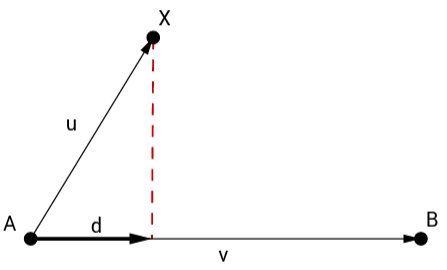
\includegraphics[scale=0.38]{images/ortogonal_projection.png}
\end{center}
$$ d = \displaystyle \frac{\langle X-A,B-A \rangle}{||B-A||} \cdot (B-A)$$

¿Cuál es el punto destino del vector $d$? Como el origen es $A$, será $d+A$.
}

\end{frame}


\begin{frame}{Encontrar centro de circunferencia a partir de tres puntos}

Supongamos que tenemos tres puntos cualquiera sobre una circunferencia. 
¿Cómo puedo hallar el centro y radio de la circunferencia?

\bigpause
\invisible<1>{
\begin{center}
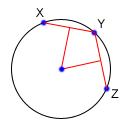
\includegraphics[scale=0.6]{images/center_circle.png}
\end{center}

Debemos hallar la intersección de las dos rectas perpendiculares a $XY$ e
$YZ$ respectivamente. Dicha intersección es el centro de la circunferencia.
Luego, $OX$ será el radio.
}
\end{frame}


\section{\'Area de un pol\'igono}

\begin{frame}{\'Area de un tri\'angulo}
Como podrán imaginar, hallar el área de un polígono es de vital relevancia
en geometría computacional. ¿Cómo podemos hallarla?

\bigpause
\invisible<1>{
Comencemos de lo m\'as sencillo: primero pensemos c\'omo sacar\'iamos el \'area de un tri\'angulo.
} 
\bigpause

\invisible<1-2>{
Recordemos lo que vimos hace un rato: si $u$ y $v$ son dos vectores que forman un \'angulo $\theta$, $|u \times v|$ es igual al \'area del paralelogramo que forman.

\begin{center}
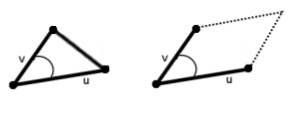
\includegraphics[scale=0.6]{images/producto_cruz_triangulo.png}
\end{center}
}
\end{frame}

\begin{frame}

As\'i, el \'area del tri\'angulo marcado es $\displaystyle\frac{|u\times v|}{2}$.\bigpause

\invisible<1>{
¿C\'omo podemos aplicar lo ya visto para sacar el \'area de un pol\'igono? 
}

\bigpause

\invisible<1-2>{
¡Triangulando! Ve\'amoslo.
}
\end{frame}

\begin{frame}{\'Area de un polígono}

Se triangula desde un v\'ertice cualquiera y se suman \textbf{en orden} 
los productos cruz. La superficie del pol\'igono es la mitad del valor 
absoluto de este n\'umero.

\begin{center}
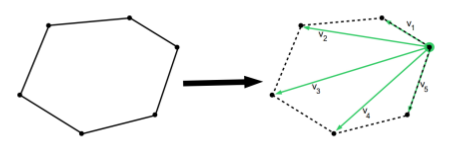
\includegraphics[scale=0.6]{images/triangulacion.png}
\end{center}

Si el pol\'igono es c\'oncavo, sigue valiendo el mismo algoritmo.
\bigpause

\invisible<1>{
Complejidad: $O(n)$ si $n$ es la cantidad de v\'ertices del pol\'igono.
}
\end{frame}

\begin{frame}
Veamos por qué sigue funcionando el mismo algoritmo para polígonos
cóncavos. Lo haremos a través de un ejemplo, pero vale en general.

\begin{center}
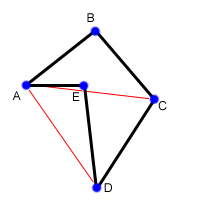
\includegraphics[scale=0.6]{images/area_polygon.png}
\end{center}
\end{frame}

\begin{frame}
Como la cuenta del área con producto cruz es con signo (puede ser negativa
o positiva según el orden de los puntos), cuando contamos un triángulo que
no está realmente en el polígono, como se invierte el orden de los puntos
se invierte el signo del área: así, se cancela lo ya sumado por otros triángulos.
\bigskip

Por ejemplo, triangulando desde $A$ se tiene:
{\small
$AreaProdCruz(ABC) + AreaProdCruz(ACD) + AreaProdCruz(ADE) = Area(ABC) + Area(ACD) - Area(ADE)$
}

\bigskip
O depende el orden como se tomen los puntos será lo mismo pero con signo inverso. Es por eso
que tomamos valor absoluto.
\end{frame}

\begin{frame}[fragile]
\footnotesize
AreaPoligono toma un arreglo listando los vértices del polígono en orden
(ya sea horario o antihorario) y calcula el área.

\begin{verbatim}
AreaPoligono (vector<punto> p){
    // Triangularemos el poligono en triangulos formados 
    // por los puntos p[0], p[i], p[i+1]
    
    area = 0
    N = cantidad de puntos en p

    for i = [1..N-1):
        x1 = p[i].x - p[0].x
        y1 = p[i].y - p[0].y
        x2 = p[i+1].x - p[0].x
        y2 = p[i+1].y - p[0].y
        area += x1 * y2 - x2 * y1
    
    devolver |area / 2.0|
}
\end{verbatim}

Notar que si las coordenadas son enteras, el área es un semientero.
\end{frame}

\section{Teorema de Pick}
\begin{frame}{Problema: City blocks}
La ciudad donde vivimos tiene forma de grilla cuadriculada. Hay $N$ calles
corriendo en sentido $sur-norte$ y $M$ calles corriendo en sentido $este-oeste$.
Un helicóptero salió de la esquina más al suroeste y voló en línea recta
hasta la esquina ubicada más al noreste. ¿Por cuántas manzanas voló el
helicóptero?

\begin{center}
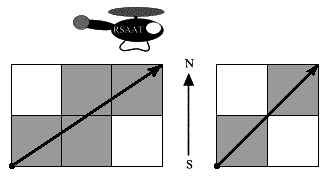
\includegraphics[scale=0.6]{images/city_blocks.png}
\end{center}

{\scriptsize Fuente: \texttt{http://acm.timus.ru/problem.aspx?space=1\&num=1139}}
\end{frame}

\begin{frame}{Teorema de Pick}

{\footnotesize
\begin{itemize}
\item $A$ es el \'area del pol\'igono.
\item $I$ es la cantidad de puntos interiores sobre la grilla.
\item $B$ es la cantidad de puntos del borde que se encuentran sobre la grilla. 
Se pueden calcular usando el MCD de la longitud en $x$ y en $y$ de cada lado.
\end{itemize}

$$ A = I + \displaystyle \frac{B}{2} -1 $$}

\begin{center}
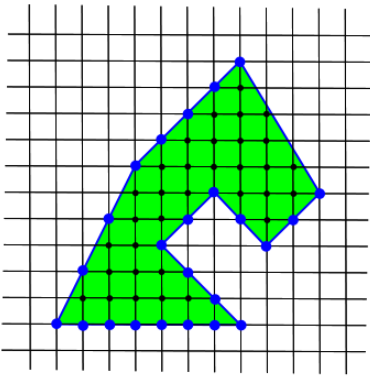
\includegraphics[scale=0.3]{images/pick.png}
\end{center}

\end{frame}

\begin{frame}{Hallar la cantidad de puntos dentro de un polígono}

Dado un polígono con todos sus vértices sobre la grilla, queremos ver
cuántos puntos de la grilla se encuentran en su interior. \textquestiondown Cómo lo
podemos hacer?

\bigpause
\invisible<1>{
$A$ ya lo sabemos calcular (área de un polígono). \\

\bigpause
\invisible<1-2>{
$B$ lo podemos calcular usando la técnica del problema anterior (MCD).

Así, despejamos $I$:

$$ A - \displaystyle \frac{B}{2} + 1 = I $$
}
}
\end{frame}

\section{Point in polygon}
\begin{frame}{Ver si un punto está dentro de un polígono}

Supongamos que nos dan un polígono (potencialmente cóncavo). Queremos
saber si un cierto punto se encuentra dentro del polígono o fuera de él.
¿Cómo podemos saberlo? 

En general, esta tarea es fácil para un humano pero no lo es para la
computadora. Este problema es conocido como \textit{Point in polygon}. 
\end{frame}

\begin{frame}
Si queremos saber si $X$ está dentro del polígono o no, podemos
buscar un punto $P$ que sabemos que seguro está fuera del polígono
y tirar un rayo en dirección $PX$. Contaremos la cantidad de cruces con
el borde del polígono, y eso determinará si el punto cayó dentro o fuera.

Gráficamente,

\begin{center}
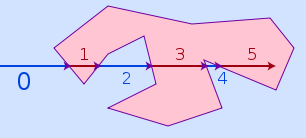
\includegraphics[scale=0.6]{images/point_in_poly.png}
\end{center}

\end{frame}

\begin{frame}{¡Hasta la semana que viene!}
\begin{center}

\includegraphics[scale=0.7]{images/to_be_continued.jpg}
\end{center}
\end{frame}

\end{document}
